\documentclass{article}
\usepackage[utf8]{inputenc}
\usepackage{amsmath}
\usepackage{hyperref}
\usepackage{listings}
\usepackage{color}
\definecolor{dkgreen}{rgb}{0,0.6,0}
\definecolor{gray}{rgb}{0.5,0.5,0.5}
\definecolor{mauve}{rgb}{0.58,0,0.82}
\lstset{frame=tb,
  language=Python,
  aboveskip=3mm,
  escapechar=\%,
  belowskip=3mm,
  showstringspaces=false,
  columns=flexible,
  basicstyle={\small\ttfamily},
  numbers=none,
  numberstyle=\tiny\color{black},
  keywordstyle=\color{black},
  commentstyle=\color{dkgreen},
  stringstyle=\color{black},
  breaklines=true,
  breakatwhitespace=true,
  tabsize=3
}
\usepackage{amsthm}
\usepackage{amssymb}
\usepackage{graphics}
\usepackage{graphicx}
\usepackage{mathtools}
\usepackage{booktabs}
\DeclareMathOperator\dom{dom}
\DeclareMathOperator\vphi{\varphi}
\DeclareMathOperator\eps{\epsilon}
\DeclareMathOperator\del{\delta}
\DeclareMathOperator\Del{\Delta}
\DeclareMathOperator\deq{\vcentcolon=}
\DeclareMathOperator\R{\mathbb{R}}
\DeclareMathOperator\Z{\mathbb{Z}}
\DeclareMathOperator\N{\mathbb{N}}
\DeclareMathOperator\F{\mathbb{F}}
\DeclareMathOperator\A{\mathbb{A}}
\DeclareMathOperator\HH{\mathbb{H}}
\DeclareMathOperator\minn{\text{Minimise} \quad }
\DeclareMathOperator\maxx{\text{Maximise} \quad }
\DeclareMathOperator\st{\text{Subject to} \quad }
\DeclareMathOperator\nc{\text{no constraints}}
\DeclarePairedDelimiter\ceil{\lceil}{\rceil}
\DeclarePairedDelimiter\floor{\lfloor}{\rfloor}
\DeclareMathOperator\bx{\bold{x}}
\DeclareMathOperator\bs{\bold{s}}
\DeclareMathOperator\bb{\bold{b}}
\DeclareMathOperator\bA{\bold{A}}
\DeclareMathOperator\bp{\bold{p}}
\DeclareMathOperator\bc{\bold{c}}
\DeclareMathOperator\C{\mathbb{C}}
\DeclareMathOperator\ran{ran}
\DeclareMathOperator\op{\oplus}
\DeclareMathOperator\ot{\otimes}
\DeclareMathOperator\diam{diam}
\DeclareMathOperator\ite{int}
\DeclareMathOperator*{\argmax}{arg\,max}
\DeclareMathOperator*{\argmin}{arg\,min}
\DeclareMathOperator\cd{card}
\DeclareMathOperator\la{\langle}
\DeclareMathOperator\ra{\rangle}

\newcommand{\seq}{(x_n)_{n \geq 1}}
\newcommand{\sseq}{(x_{n_k})_{k \geq 1}}
\newcommand{\fseq}{(f_n)_{n \geq 1}}
\newcommand{\elll}{\ell^{\infty}(\N)}
\newcommand{\norm}{{\|.\|}}
\newcommand{\inner}{\langle .,. \rangle}

\usepackage{color}
\title{MATH310}


\begin{document}
\maketitle{}
\newpage{}

\section*{Cardinality (Mostly week 1)}
\subsection*{Definition: Finite Cardinality}
The set $\emptyset$ has a finite cardinality of zero. A set $A \neq \emptyset$ is finite if there is a bijection between $A$ and $\{1,\hdots,n \}:n \in \N$. If not,
$A$ is said to be infinite.
\subsection*{Definition: Lesser Cardinality}
We have $\cd(A) \leq \cd(B)$ if there is a one to one map between $A$ and $B$.
\subsection*{Theorem: Infinite Cardinality}
A set $A$ is infinite iff $\exists B \subsetneq A: \cd(A) = \cd(B)$.
\subsubsection*{Lemma: Infinite set contains a denumerable set}
Let $A$ be an infinite set with $a_1 \in A$. We claim that $A \backslash a_1$ is also an infinite set. Suppose not. Then
$A \backslash a_1$ is a finite set and there is a bijection $\phi: A \backslash a_1 \to \{1, \hdots, n \}$ for some $n \in \N$.
Define $\psi:A \to \{1, \hdots,n+1 \}$, $$
\psi(x) = \begin{cases}
n+1, \quad x = a_1 \\
\phi(x), \quad x \neq a_1.
\end{cases}
$$
Fill in details using onto and one to one property of $\phi$. So $A \setminus \{a_1\}$ is also an infinite set.
Hence $A \setminus \{ a_1, \hdots \}$ is infinite and so $A$ contains a denumerable subset.
\subsubsection*{$(\implies)$}
Hilbert hotel.
\subsubsection*{$(\impliedby)$}
Suppose $B \subsetneq A$ and $\cd(A) = \cd(B)$. We claim that $A$ is infinite. We prove a lemma:
\begin{proof}
Suppose $f: \{1,\hdots,n \} \to \{1,\hdots,n \}$ is injective.
We claim that $f$ is bijective. We prove by induction, base case is obvious.
Let $f:\{1,\hdots,n +1 \} \to \{1,\hdots,n +1 \}$ be an injective function.
Define $s:\{1,\hdots,n+1 \} \to \{1,\hdots,n+1 \}$,$$
s(k) = \begin{cases}
k, \quad k \neq n+1,f(n+1) \\
n+1, \quad k = f(n+1) \\
f(n+1), \quad k = n+1.
\end{cases}
$$
Conveniently, $s^{-1} = s$ and $s$ is bijective (but inverse of a bijection is bijective anyway). So $s \circ f \vert_{1,\hdots,n}$ is injective (composition of 1:1 is 1:1)
and surjective (by supposition). Since $s \circ f(n+1) = n+1$, the function $s \circ f$ is one to one and onto.
So $f = s^{-1} \circ s \circ f$ is bijective (composition of bijective functions is bijective). Done by induction.
\end{proof}
\noindent And now for something completely the same ...
\begin{proof}
There is a bijection $f:A \to B$ cause $\cd(A) = \cd(B)$.
The inclusion map $\iota: B \hookrightarrow A$
is one to one but not onto (proper subset). So $\iota \circ f$ is 1:1 not onto. Suppose for a contradiction that $A$
is finite. Then there is a bijection $g:A \to \{1,\hdots,n \}$
and another bijection $g^{-1}$. So we compose a bunch of
1:1 functions to get a new 1:1 function:
$$
g \circ \iota \circ f \circ g^{-1}: \{1,\hdots,n \} \to \{1,\hdots,n \}
$$

\end{proof}
\subsection*{Lemma: Any subset of a countable set is countable}
Suppose that $Q \subset A$ and $A = \{a_1,\hdots \}$ is countable. Then $B = \{ a_{j_1},\hdots \}$ where $a_{j_i} \in B \cap A$, so $B$ is countable.

\subsection*{Theorem: $\mathbb{Q}$ is denumerable (same cardinality as $\N$)}
The Calkin-Wilf sequence is a 1:1 and onto function $f:\N \to \mathbb{Q}^+$ given by $$
q_n = \begin{cases}
1, \,\, n = 1 \\
\frac{1}{1+2\floor*{q_{n-1}} - q_{n-1}}, \,\, n \neq 1
\end{cases}
$$
We can define a new sequence $q = (q_n)_{n \geq 1}$, $q_1 = 0, q_2 = 1, q_3 = -1, q_{2k+1} = -q_{2k}$ and  $$
q_{2k} = \frac{1}{1+2\floor*{q_{2k-2}} - q_{2k-2}}
$$
for $k \in \N: k \geq 2$. The function $q: \N \to \mathbb{Q}$ is bijective.
\subsection*{Theorem: Cantor's Diagonal Argument, $\cd(\N) \neq \cd(\R)$}
We claim that $(0,1)$ is not countable, so $\R$ cannot be since $M = (0,1)$ is a subset.
Suppose not. Then $M = \{r_1,\hdots \}$
with $r_n = 0.a_{n1}a_{n2}\hdots$ (chosen uniquely as the expansion
without zeros at the end) with $a_{ni} \in \{0,\hdots,9\}$. Define $b_k = \min\{ x \in \{ 1,2\}: x \neq a_{nk} \}$
and $b = 0.b_1\hdots$ so that $b \in (0,1)$ and $b \neq r_p \forall p \in \N$
since $b_p \neq a_{pp}$.
\subsection*{Theorem: $0 < 1 < \hdots < d < c$}
\subsection*{Axiom: Choice}
\subsubsection*{Theorem: $\exists$ surjection $B \to A$ $\iff$ $\exists$ injection $A \to B$}
\subsection*{Choice-Equivalent-Axiom: Zorn's Lemma}
\paragraph{Definition: Binary Relation}
A binary relation on a set $X$ is any subset $R \subset X \times X$. We write $x \sim y$ as an abbreviation of $(x,y) \in R$.
\paragraph{Definition: Partial Ordering}
A partial ordering on a set $X$ is a binary relation that respects reflexivity, anti-symmetry and transitivity.
\paragraph{Definition: Chain}
Suppose there is a partial ordering $\leq$ on a set $X$ and $Q \subset X$. Then
the partial ordering on $Q$ is called a total ordering if $\forall \,\, (x,y) \in Q$, $x \leq y$ or $y \leq x$. In this case we call $Q$ a chain.
\paragraph{Maximal and Maximum are different without a total ordering}
A point $x \in X$ is maximal if $\forall y \in X$, $x \leq y \implies x=y$. The same point is a maximum if $\forall y \in X$, $y \leq x$.
\paragraph{Zorn's Lemma:}
Suppose $(X,\leq)$ is a poset and every chain $Q \subset X$ has an upper bound.
Then $X$ has a maximal element.
\subsubsection*{Shroder-Bernstein Theorem (Trichotomy $\iff$ Zorn)}
Cardinals obey reflexivity, anti-symmetry and transitivity WRT $\leq$,
trichotomy and commute with equality.
\subsubsection*{Every vector space has a basis}

\subsection*{Exercises}
\subsubsection*{Lemma: Cartesian product of sets has the cardinality type of the largest set in the product}

\subsubsection*{Lemma: Countable/uncountable union of countable/uncountable sets is countable/uncountable}

\subsubsection*{Lemma: The set of finite subsets of $\N$ is countable}

\subsubsection*{Lemma: The set of infinite subsets of $\N$ is uncountable}

\subsection*{Theorem: Power sets have greater cardinality}

\section*{Basic Metric Topology (Mostly Week 2)}
\subsection*{Every Vector Space has a Basis}
\subsection*{Metric Definition}
\subsection*{Norm Definition}
\subsection*{Types of points in a set}
\subsubsection*{Balls around interior pts of $A \subset X$ are subsets of $A$ if small enough}
\subsubsection*{Balls around exterior pts of $A \subset X$ are subsets of $A^c$ if small enough}
\subsubsection*{Balls around limit points of $A \subset X$ contain different points in $A$ no matter the size of ball}
\subsection*{Typical results of complements, exteriors, unions and intersections}
\subsection*{Lemma}
Let $A \subset X$ and $S \subset A$. Then $S$ is open in $A$ iff $\exists U$ open in $X$ such that $S = A \cap U$.
\begin{proof}
https://math.stackexchange.com/questions/66279/intersection-distributing-over-an-infinite-union-union-over-an-infinite-interse
\begin{center}
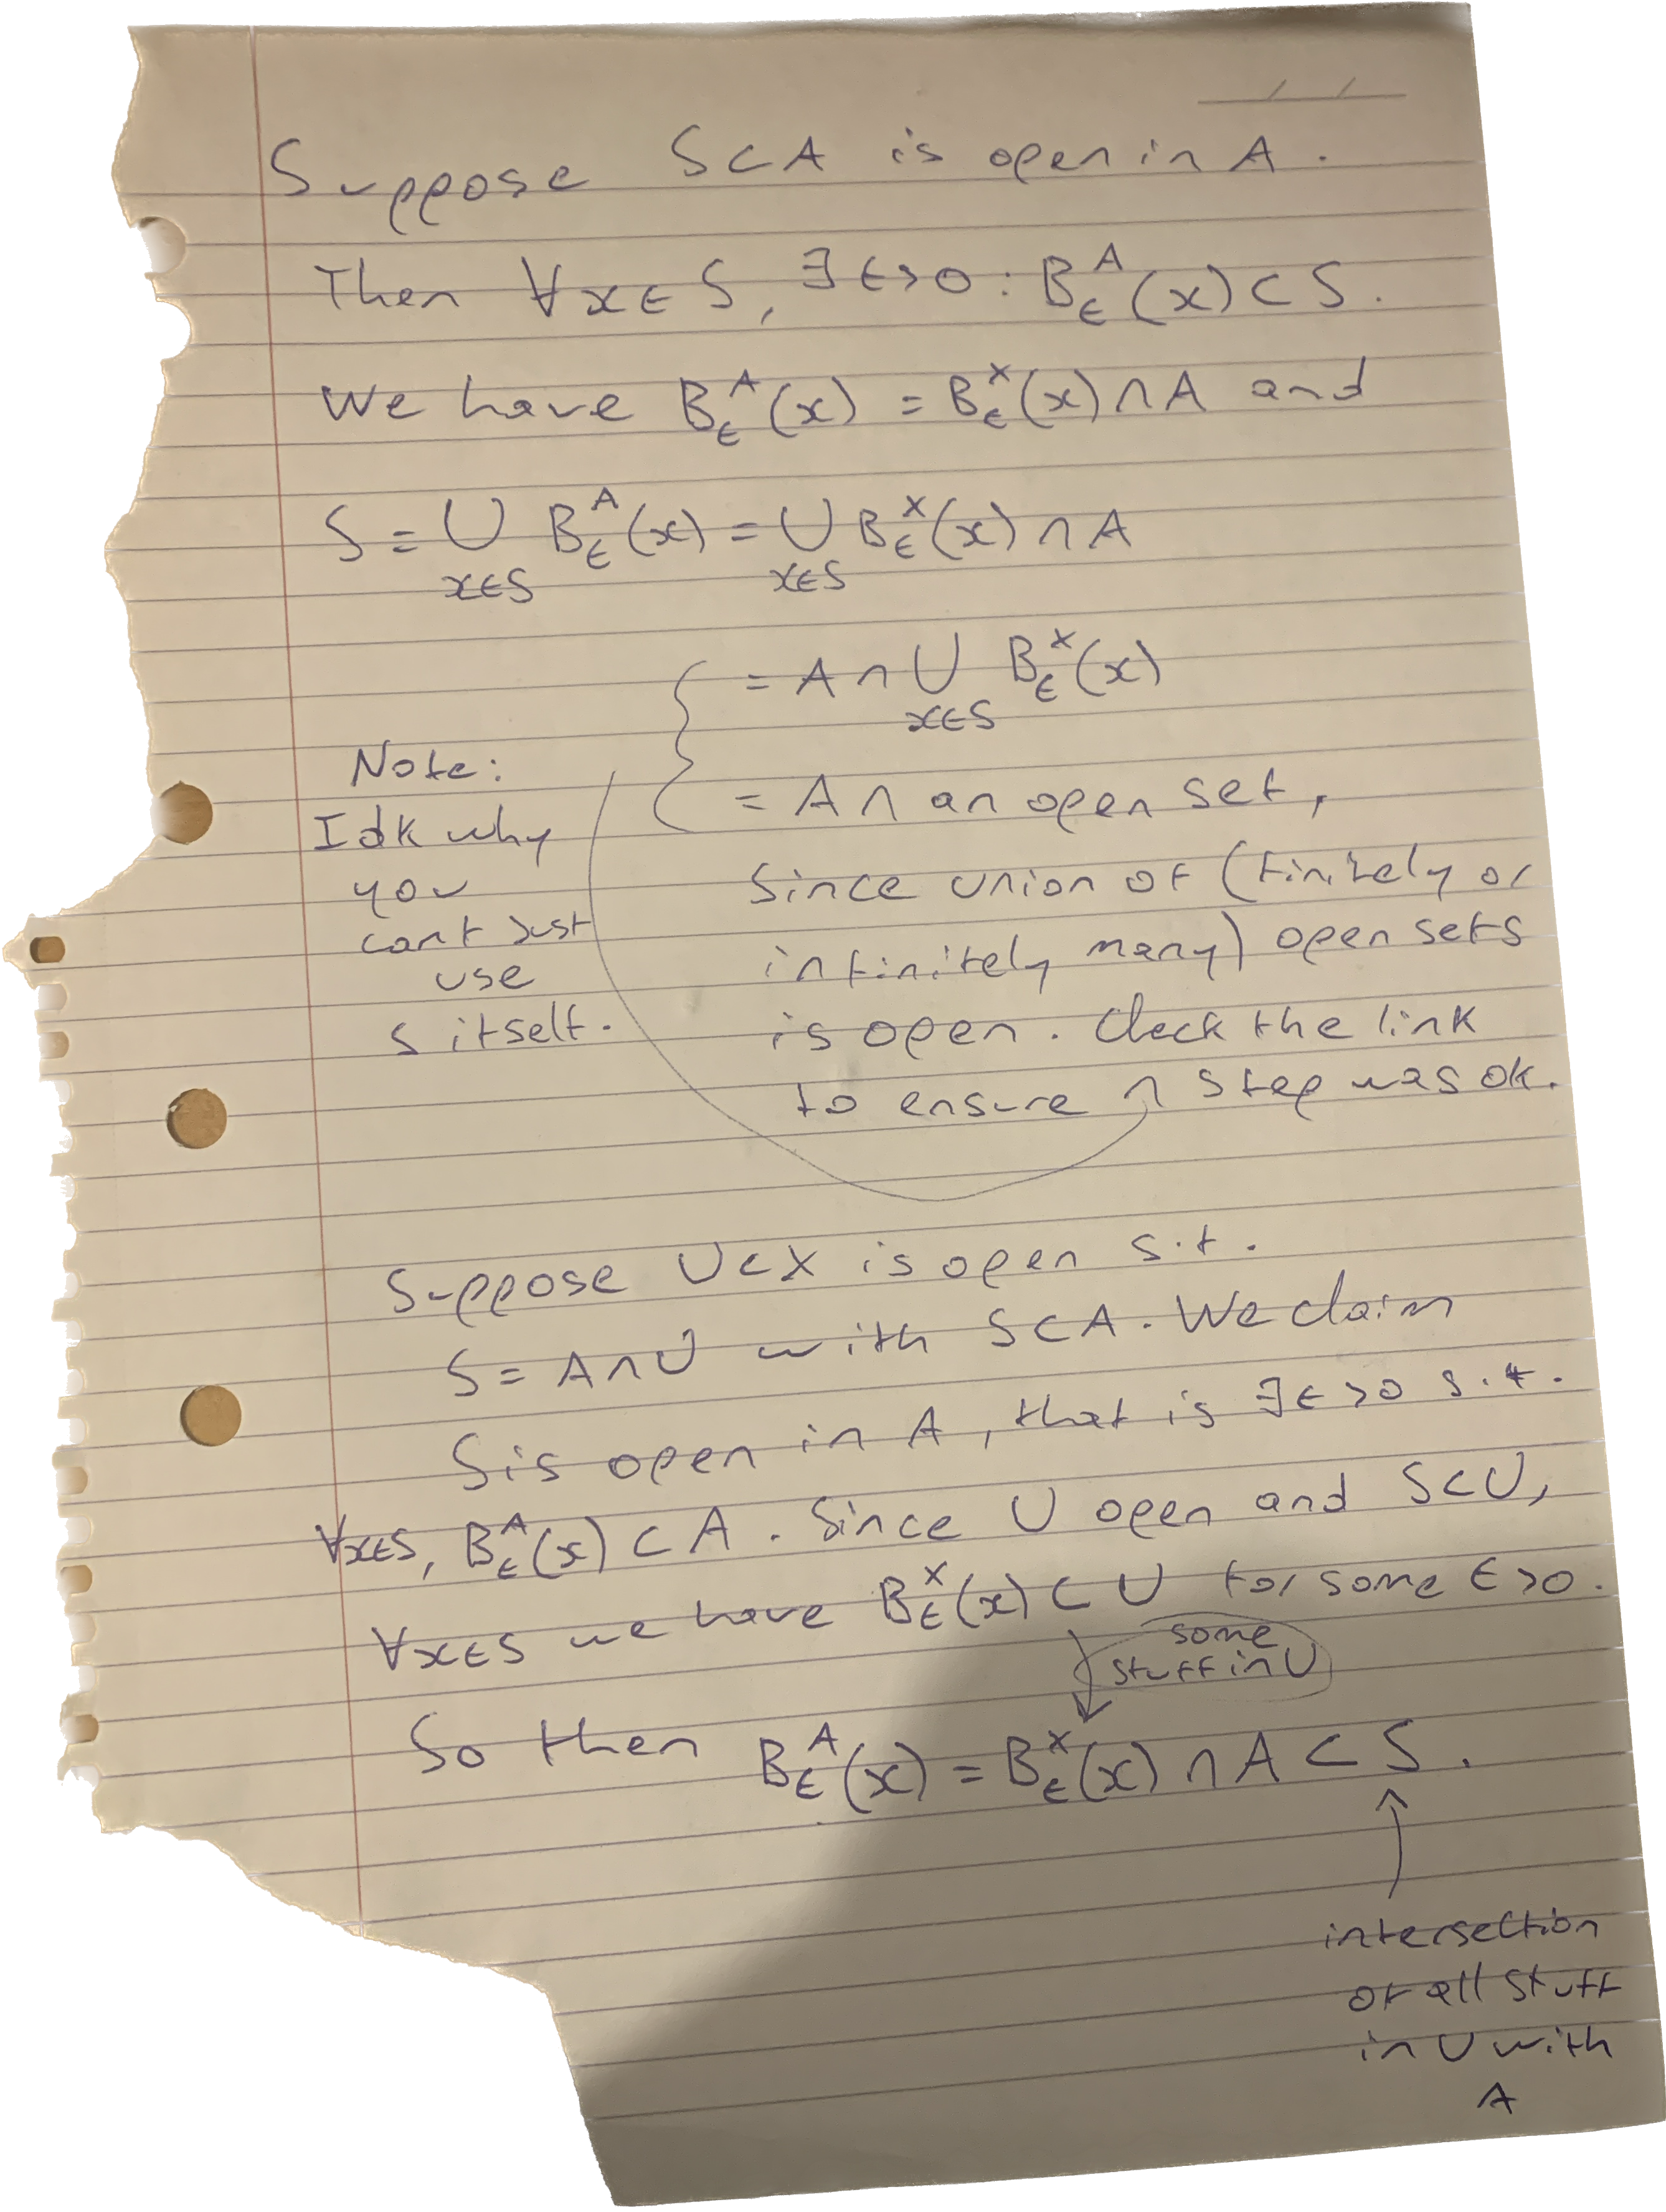
\includegraphics[scale=0.1, angle=-0]{fig/Subject.png}
\end{center}
A corollary is that the same works for closed sets. Suppose $S \subset A$ is closed. Then $S^c \subset A$ is open and
from the prior proof
$$\exists U \subset X: \text{ $U$ is open in $X$ and } S^c = A \cap U.$$
But then $S = A \setminus S^c = A \cap U^c$ in $X$ and $U^c$ is closed as it is the complement of an open set. Conversely
if $U$ is closed, $S \subset A$ and $S = A \cap U$ then $S^c \subset A$ and $S^c = A \cap U^c$ so we must have $S^c$ open from the prior and hence $S$ is closed. This is called the
\textbf{inheritance principle}.
\end{proof}
\subsection*{Definition}
The diameter of a set $A \subset X$ is given by
$$
\diam(A) = \sup \{ d(x,y):x,y \in A \}.
$$
We say that $A$ is bounded if $\diam(A) < \infty$. Equivalently, $\exists x \in X$, $r>0: A \subset B_r(x)$.
\subsection*{Lemma}
Suppose $(X,d)$ is a MS and $A \subset X$ is bounded. Then $\forall y \in Y$, $$
\exists \rho > 0: A \subset B_{\rho}(y).
$$
\begin{proof}
Fix $y \in Y$, $a \in A$. Since $A$ is bounded,
there is some $x \in X$, $r>0$
such that $d(a,x) < r$. Set $\rho = d(x,y) + r$. Then $$
d(a,y) \leq d(a,x) + d(x,y) = r + d(x,y)
$$
and so $a \in B_{\rho}(y)$. So $A \subset B_{\rho}(y)$.
\end{proof}
\subsection*{Convergence of sequences and uniqueness of convergence}
\section*{Equivalent and Complete Metric Spaces (Start of Week 3)}
\subsection*{Definition: Equivalent Metrics}
Suppose that $(X,d_1),(X,d_2)$ are metric spaces.
We say that $d_1$ and $d_2$ are
equivalent if for any sequence $(x_n)_{n \geq 1}$ we have $$
x_n \to^{d_1} x_0 \in X \iff x_n \to^{d_2} x_0.
$$
\subsubsection*{Lemma $(\star)$}
Suppose $\exists \alpha,\beta > 0: \forall x,y \in X$ we have $$
\beta d_1(x,y) \leq d_2(x,y) \leq \alpha d_1(x,y).
$$
Then $d_1$ and $d_2$ are equivalent metrics on $X$.
\subsubsection*{Lemma}
Suppose there exists a strictly increasing continuous function
$f: \R \to \R^{+}$
that satisfies
$$
f(x+y) \leq f(x) + f(y) \quad \forall x,y \in X
$$
and $$
d_2 = f(d_1).
$$
Then $d_1$ and $d_2$ are equivalent metrics on $X$.
\subsection*{Definition}
Suppose that $(X,{\|.\|}_1)$ and $(X,{\|.\|}_2)$ are normed metric spaces.
Then ${\|.\|}_1$ and ${\|.\|}_2$ are equivalent iff $(\star)$ holds.
That is, bi-Lipshitz equivalence holds iff regular
(topological) equivalence holds,
for metrics that induce a norm. Note: bi-Lipshitz is used here WRT the metrics, rather than the spaces, but the term can apply to both.
\subsection*{Definition: Equivalent Spaces}
Suppose that $(X,d_1),(Y,d_2)$ are metric spaces.
We say that $X$ and $Y$ are
bi-Lipshitz equivalent if there exist constants
$c_1,c_2 > 0$ and a bijective function $f: X \to Y$ such that
$\forall x,y \in X$ and $w,z \in Y$$$
|f(x)-f(y)| \leq c_1 d_1(x,y)
$$
and $$
|f^{-1}(w)-f^{-1}(z)| \leq c_2 d_2(w,z).
$$
\subsubsection*{Non-example}
The spaces $(C([0,1]),\norm_1)$ and $(C([0,1]),\norm_{\infty})$ are not equivalent.
Choose $\fseq$, $f_n(x) = x^n$. Then ${\|f_n\|}_{\infty} = 1 \to 1$ but ${\|f_n\|}_1 = \int_0^1 x^n dx = \frac{1}{n+1} \to 0 \neq 1$.
\subsection*{Theorem}
Suppose that $V_1 = (V,\norm_1), V_2 = (V,\norm_2)$
are normed vector spaces and $\norm_1,\norm_2$ are equivalent.
Then $V_1$ and $V_2$ are bi-Lipshitz equivalent.
\begin{proof}
Since $\norm_1$ and $\norm_2$ are equivalent,
we have that
$$
\exists \alpha > 0: \frac{1}{\alpha} {\|x\|}_1 \leq {\|x\|}_2 \leq \alpha {\|x\|}_1.
$$
for each $x \in V$. Define $f:V \to V$,
$$
f(x) = x \implies f^{-1}(x) =
x.
$$
Then $$
{\|f(x)-f(y)\|}_2 = {\|x-y\|}_2 \leq \alpha {\|x-y\|}_1
$$
and
$$
{\|f^{-1}(w)-f^{-1}(z)\|}_1 = {\|w-z\|}_1 \leq \alpha {\|w-z\|}_2
$$
\end{proof}
\subsection*{Definition}
A metric space is complete iff every Cauchy sequence converges to a limit.
\subsection*{TODO this is equivalent to a vairant of cantors intersection theorem}
\subsubsection*{Non-example}
The space $(c_{00}(\N),\norm_{\infty})$ with $$
c_{00}(\N) = \{ \seq : x_n \in \C, \exists Q \in \N: \forall n \geq Q, x_n =0 \}.
$$
Define a sequence of points in $c_{00}$, $X = ((x_n)^k_{n \geq 1})_{k \geq 1}$,
with
$$
(x_n)^k_{n \geq 1}: x_n^k = \begin{cases}
\frac{1}{n}, & n \leq k \\
0, & n > k.
\end{cases}
$$
Fix $\eps>0$.
By the Archimedean property, $\exists N \in \N: N > 1 \slash \eps$.
Then for sequences $y^k,y^j: j \geq N, k > j$ we have
$$
{\|y^k-y^j\|}_{\infty} = \max \left \{ \frac{1}{j+1}, \frac{1}{j+2},
\hdots, \frac{1}{k} \right \}  = \frac{1}{j+1}  < \eps.
$$
So $X$ is Cauchy. Fix $L \in C_{00}(\N)$ and $N \in \N$.
By definition of $L$, the set $Y = \min \{ R \in \N: \forall k \geq R, L_k = 0 \} \not = \emptyset$
and so it has a least element, call it $Q$.
Let $H = \max \{N+1,Q\}$. For $k \geq H$ we have
$$
{\|y^k-L\|}_{\infty} = \max \left \{ \frac{1}{H}, \hdots, \frac{1}{k} \right \} \geq \frac{1}{H} > 0.
$$
So $X \not \to L$ and hence $c_{00}(\N)$ is not complete.
Also $\R^k$ missing any point is not complete in the standard metric. But not in general, every discrete metric space is complete.
\subsection*{Theorem}
Suppose that $(X,d)$ is a complete metic space and $A \subset X$. Then $(A,d {\vert_A})$ is complete iff $A$ is closed.
\begin{proof}
Suppose $A \subset X$ is closed and $\seq \subset A$ is Cauchy.
Then $\seq$ converges in $X$ and since closed sets contain their limit points
we have that $\seq$ converges in $A$. \\ \newline
Suppose $(A, d \vert_A)$ is complete and $\seq$ converges in $X$.
Then $\seq$ is Cauchy, so it converges in $A$ also and hence $A$ is closed.
\end{proof}
\subsection*{Definition}
A Banach space is a complete and normed vector space.
\section*{Convexity, Holder, Minkowski, $L_p$ spaces, $C$ spaces, Hilbert spaces (Rest of Week 3)}
\subsection*{Definition}
A set $C \subset \R^n$ is convex if $\forall x,y \in C, t \in [0,1]$ we have $$
tx+(1-t)y \in C. $$
Suppose $f:C \to \R$ is a function that maps a convex set. Then $f$ is convex if
$$
f(tx+(1-t)y) \leq tf(x) + (1-t)f(y)
$$
and concave if the inequality is reversed. In general functions can be both (which must be linear functions) or neither.
Any bounded and closed set in $\R$ that is convex is also a closed interval.
Open intervals in $\R$ are convex. \\ \newline Any function $f: I \to \R$ is convex iff $-f$ is concave, $f'$ is nondecreasing and $$
x \mapsto \frac{f(y) - f(x)}{y-x}
$$
is a nondecreasing function for fixed $y \in I$.
\subsection*{Theorem: Young's Inequality}
Fix $a,b \geq 0$ and $p,q: 1 < p,q < \infty$ and $\frac{1}{p}+\frac{1}{q} = 1$.
The $\log$ function is concave so for $a,b >0$ (if not then trivially done):
\begin{align*}
\log \left( \frac{a^p}{p}+\frac{b^q}{q} \right) &= \log \left( \frac{a^p}{p}+\left(1-\frac{1}{p} \right) b^q \right) \\
&\geq \frac{1}{p} \log \left( a^p \right) + \left(1-\frac{1}{p} \right) \log \left( b^q \right) \\
&= \log(ab)
\end{align*}
and so $ab \leq \frac{a^p}{p}+\frac{b^q}{q}$ since $\exp$ is increasing. We claim $a^p = b^q \iff \frac{a^p}{p}+\frac{b^q}{q} = ab$.
\begin{proof}
We have $a^p = b^q \implies \frac{a^p}{p}+\frac{b^q}{q} = \frac{(q+p)a^p}{pq} = a^p = a^{p-1}a = a^{p \slash q}a = ab$.
\\ \newline
Have a look here for the other direction: https://math.stackexchange.com/questions/566307/showing-when-youngs-inequality-is-in-fact-equality.
\end{proof}
\subsection*{Theorem: Hölder's Inequality}
Fix $x,y \in \R^n$ and $p,q: 1 < p,q < \infty$ and $\frac{1}{p}+\frac{1}{q} = 1$. We claim that $$
\sum_{i=1}^n |x_iy_i| \leq {\|x\|}_{p} {\|y\|}_{q}.
$$
\begin{proof}
We have \begin{align*}
\sum_{i=1}^n |x_iy_i| &= \sum_{i=1}^n |x_i||y_i| \\
&\leq \sum_{i=1}^n \left( \frac{|x_i|^p}{p} + \frac{|y_i|^q}{q} \right) \text{ by Young's inequality}
\\
&= \frac{1}{p}{\|x\|}_p^p +\frac{1}{q}{\|y\|}_q^q \\
&= 1 \text{ when ${\|y\|}_q = {\|x\|}_p = 1$}.
\end{align*}
So we can choose $x' = \frac{x}{\|x\|}$ and $y' = \frac{y}{\|y\|}$ to get
$$
\sum |x_i'y_i'| = \sum \left| \frac{x_i}{\|x\|}\frac{y_i}{\|y\|} \right| \leq 1 \implies \sum |x_iy_i| \leq \|x\| \|y\|.
$$
\end{proof}
\subsection*{TODO: Relations between p-norms}
https://en.wikipedia.org/wiki/Lp `underscore' space
\subsection*{TODO: $\|f+g\|_p$ is finite (see Minkowski wikipedia)}
We have $$
\|f+g\|_p = \left(\sum_{i=1}^n |f_i+g_i|^p \right)^{1 \slash p}
$$
The function $|x|^p$ for $p<1$ is convex. So $$
|0.5f+0.5g|^p \leq |0.5|f|+0.5|g||^p \leq 0.5|f|^p +0.5|g|^p
$$
\subsection*{Theorem: Minkowski's Inequality}
We claim that $\norm_p: 1 < p < \infty$ are norms on finite dimensional vector spaces. In particular, they satisfy the triangle.
\subsubsection*{Lemma (we now prove triangle inequality)}
For $p<1$, $n \in \N$ and $a_i \in \R$
we have $$
1 = \sum_{i=1}^{k+1} \frac{|a_i|}{\sum_{i=1}^{k+1} |a_i|} \leq
\sum_{i=1}^{k+1} \left( \frac{|a_i|}{\sum_{i=1}^{k+1} |a_i|} \right)^p \implies \left( \sum |a_i| \right)^p \leq \sum |a_i|^p
$$
\begin{proof}
\begin{align*}
{\|x+y\|}_p^p &= \sum_{i=1}^n |x_i+y_i|^p \\
&\leq \sum_{i=1}^n |x_i+y_i|^{p-1}(|x_i|+|y_i|) \text{ by triangle } \\
&\leq \left( \sum_{i=1}^n {|x_i+y_i|}^p \right)^{\frac{p-1}{p}}
\left( \left( \sum_{i=1}^n |x_i|^p\right)^{1 \slash p} + \left( \sum_{i=1}^n |y_i|^p \right)^{1 \slash p} \right)  \text{ by holder twice or holder once, lemma } \\
&= {\|x+y\|}_p^{p-1} ({\|x\|}_p+{\|y\|}_p) \\
\text{ and so } & {\|x+y\|}_p \leq {\|x\|}_p+{\|y\|}_p.
\end{align*}
\end{proof}
\subsubsection*{Corollaries (infinite dimensions)}
For $\Omega \subset \R^n$ and $$
\|f\|_p = \left( \int_{\Omega}|f(x)|^pd^nx \right)^{1 \slash p}
$$
we have $$
\int_{\Omega} |f(x)+g(x)|d^nx \leq {\|f\|}_p+ {\|g\|}_p
$$
and $$
\|f+g\|_p \leq \|f\|_p + \|g\|_p.
$$
\subsection*{Definitions}
\subsubsection*{$\ell$ spaces}
$$
\ell^p(\N) = \{ \seq: x_n \in \C, \quad \sum_{i=1}^{\infty} |x_n|^p < \infty \}
$$
$$
\ell^{\infty}(\N) =  \{ \seq: x_n \in \C, \quad \sup |x_n| < \infty \}
$$
\subsubsection*{$L$ spaces}
Let $\Omega \subset \R^n$ be a compact / closed and bounded set.
$$
L^p(\Omega) = \{f: \Omega \to \C, \quad \int_{\Omega}|f|^p d^nx < \infty \}
$$
$$
L^{\infty}(\Omega) = \{f: \Omega \to \C, \quad \sup_{x \in \Omega}|f(x)| < \infty \}
$$
\subsubsection*{$C$ spaces}
$$
c_0(\N) = \{ \seq: x_n \in \C, \,\, x_n \to 0 \}
$$
$$
c_{00}(\N) = \{ \seq: x_n \in \C, \,\, \text{ $x_n$ eventually zero }  \}
$$
$$
C(\Omega) = \{ f: \Omega \to \C: \,\, f \text{ is cts} \}
$$
Instead of $\Omega$ being compact, take $\Omega$ as an open subset of $\R^n$.
Let $K \subset \Omega$ be a compact set and
$K'$ be its complement in $\Omega$. Then $$
C_0(\Omega) = \{ f: \Omega \to \C: \,\, f \text{ is cts and } \forall \eps > 0 \,\, \exists K \subset \Omega: x \in K' \implies |f(x)| < \eps  \}
$$
$$
\iff \{ f: \Omega \to \C: \,\, \text{ $f$ is cts and vanishes at $\infty$}  \}
$$
$$
C_0^k(\Omega) = \{ f: \Omega \to \C: \,\, \text{ $f$ is $k$ times ctsly diffable and partials up to order $k$ vanish at $\infty$}  \}
$$
This one has a weird norm:
$$
\alpha = (\alpha_1, \hdots, \alpha_n): \alpha_i \in \N \implies \alpha \in \N^n
$$
$$
|\alpha| = \sum_{i=1}^n \alpha_i
$$
$$
\partial^{\alpha} = \frac{\partial^{|\alpha|}}{\sum_{i=1}^n \partial x_i^{\alpha_i}}
$$
$$
\|f\|_k = \sum_{0 \leq |\alpha| \leq k} {\|\partial^{\alpha}f\|}_{\infty}
$$
\subsection*{Definition}
A Hilbert space is a complete inner product space. The Hermitian inner product defines a norm via
$$
\|v\| = \sqrt{\la v,v \ra}
$$
and Cauchy-Schwarz $$
\la v,w \ra \leq \|v\| \|w\|
$$
\subsubsection*{Examples}
$$
L^2(\Omega) \text{ with } \la f,g\ra =\int_{\Omega}
\overline{f(x)}g(x)d^nx
$$
$$
\ell^2(\N) \text{ with } \la x,y\ra = \sum_{i=1}^{\infty} \overline{x_i}y_i
$$
$$
\C^n \text{ with } \la x,y \ra = \sum_{i=1}^n \overline{x_i}y_i
$$
\subsection*{TODO: Subspace relations}
Prove the following subspace relations
$$C(\Omega) \subset L^{\infty}(\Omega)$$, $$c_{00}(\N) \subset c_0(\N)$$,
$$
c_0(\N) \subset \ell^{\infty}(\N)
$$
and check $C_0$ sup norm makes sense. \\ \newline
\subsubsection*{Proofs}
First one: continuous functions on compact sets are bounded so its a subset. Subspace bit is easy.
Second one: Obvious. Third one: Every convergent sequence is bounded so its a subset.
\section*{Completion of a metric space, Equivalence Classes (Start of week 4)}
\subsection*{Definition}
An equivalence relation is a binary relation $\sim$ on a set $X$. That is a subset of $X \times X$ that is reflexive, transitive and symmetric in the ordered pairs.
\subsection*{Definition}
The equivalence class of a point $x_0 \in X$ is the set
$$
\{x \in X: x \sim x_0 \}.
$$
The equivalence classes of $X$ can be used to construct a set called a partition of $X$.
That is, a collection of nonempty and disjoint subsets with union $X$. This partition is referred to as the quotient space of $X$ by $\sim$ and is denoted $X \slash \sim$. \\ \newline
An example is the relation on $\Z$ given by $x \sim y$ iff $x-y$ is even.
Clearly $2k \sim 2m$ and $2k+1 \sim 2m+1$ but $2k \not \sim 2m+1$ for
any integers $k,m$.
So there are two equivalence classes, the even and odd numbers
which are nonempty and disjoint with union $\Z$.
\subsection*{Theorem: Every Metric Space has a Completion}
Suppose that $(X_0,d_0)$ is a metric space. Then there exists
another metric space $(X,d)$ which satisfies the following:
$$
d \vert_{X_0} = d_0, \,\, \exists \iota: X_0 \hookrightarrow X, \,\, \forall x \in X, \,\, \exists \seq \subset X_0: x_n \to x \text{ as } n \to \infty.
$$
\begin{proof}
Let $Y = \{ \seq \subset X_0: \seq \text{ is Cauchy} \}$.
Define an equivalence relation on $Y$ with
$\seq \sim (y_n)_{n \geq 1}$ iff $d_0(x_n,y_n) \to 0$ as $n \to \infty$.
First we check transitivity. Suppose $\seq \sim (y_n)_{n \geq 1}$
and $(y_n)_{n \geq 1} \sim (z_n)_{n \geq 1}$. Then $$
d_0(x_n,z_n) \leq d_0(x_n,y_n) + d_0(y_n,z_n) \to 0 \text{ as }
n \to \infty.
$$
Next we check reflexivity. $$
d_0(x_n,x_n) = 0 \to 0 \text{ as } n \to \infty.
$$
Finally we check the relation is symmetric, which is true because the distance function is. \\ \newline
Let $X = Y \slash \sim$ and $d( [ \seq ], [ (y_n)_{n \geq 1} ]) =
 \lim_{n \to \infty} d_0(x,y)$ for any sequences $x,y$ in the respective
 equivalence classes. \\ \newline We check $d$ is well defined by
taking $(x_n),(q_n) \in [\seq]$ and $(w_n),(z_n) \in [(y_n)]$ and using triangle twice to get $$
\lim_{n \to \infty} d_0(x_n,w_n) \leq \lim_{n \to \infty} d_0(q_n, z_n), \,\, \lim_{n \to \infty} d_0(x_n,w_n) \geq \lim_{n \to \infty} d_0(q_n, z_n)
$$
and so they are equal and the choice of $x,y$ in $[\seq],[(y_n)]$ was irrelevant. \\ \newline
We check $d$ is indeed a metric. Suppose $[(x_n)] = [(y_n)]$.
Then choose $x \in [(x_n)]$ and $y \in [(y_n)] = [(x_n)]$
so that $d( [ \seq ], [ (y_n)_{n \geq 1} ]) = \lim_{n \to \infty} d_0(x_n,y_n)$.
Then $d( [ \seq ], [ (y_n)_{n \geq 1} ]) = \lim_{n \to \infty} d_0(x_n,y_n) = 0$
since $x \sim y$. Suppose $d( [ \seq ], [ (y_n)_{n \geq 1} ]) = 0$. Then $x \sim y$ and so for any $q \in [(x_n)]$ we have
$q \sim x \sim y$ and so by transitivity $q \sim y$ and hence $[(x_n)] \subset [(y_n)]$ and similarly $[(y_n)] \subset [(x_n)]$.
Other two are boring. Note that these limits exist because distance between Cauchy sequences in any metric space are convergent in $\R$.
\begin{center}
\includegraphics[scale=0.05, angle=-90]{fig/fred1.JPG}
\includegraphics[scale=0.05, angle=-90]{fig/fred2.JPG}
\end{center}
\end{proof}
\section*{Contraction Mapping theorem, Hausdorff and Fractals (Mostly week 4)}
\subsection*{Definition}
Let $(X,d)$ be a MS and $A \subset X$. A function $$
f: A \to X
$$
is said to be a contraction if $\exists \lambda \in [0,1)$ such that $$
d(f(x),f(y)) \leq \lambda d(x,y)
$$
for all $x,y \in A$. We say that
$x_0 \in A$ is a fixed point of $f$ if $f(x_0) = x_0$. The `fixed point' is a point in the general sense of the word, element, it could be a set or some such.
\subsection*{Contraction Mapping Theorem}
Suppose $(X,d)$ is a complete MS and $f$ is a contraction on $X$. Then $$
\exists! x_0 \in X: f(x_0) = x_0.
$$
\begin{proof}
Fix $\eps>0$.
Fix a contraction $f$ with contraction ratio $\lambda \in [0,1)$.
Choose some $x_0 \in X$ and set $x_n = f(x_{n-1})$. Choose $N \in \N$
such that $N > \log_{\lambda} \left( \frac{(1-\lambda)\eps}{d(x_0,x_1)} \right)$ so that (Note: $N \mapsto \lambda^N$ is a decreasing function) we get what we need.
Then \begin{align*}
d(x_n,x_m) &\leq d(x_n,x_{n+1}) + \hdots + d(x_{m-1},x_m) \\
&= d(f(x_{n-1}),f(x_n)) + \hdots + d(f(x_{m-2}),f(x_{m-1})) \\
& \leq \lambda d(x_{n-1},x_n) + \hdots + \lambda d(x_{m-2},x_{m-1}) \\
&\vdots \\
&\leq \lambda^n d(x_0,x_1) + \hdots + \lambda^{m-1}d(x_0,x_1) \\
&= \lambda^n(1+\hdots+\lambda^{m-1-n})d(x_0,x_1) \\
& \leq \lambda^n \slash (1 - \lambda) \times d(x_0,x_1)
< \eps.
\end{align*}
So the sequence $\seq$ is Cauchy with limit $L \in X$. Then \begin{align*}
d(L,f(L)) &\leq d(L,x_n) + d(x_n,f(L)) \\
&\leq \eps + \lambda d(x_{n-1},L) \\
& \leq 2 \eps.
\end{align*}
for large enough $n$ since $\seq$ converges to $L$. So $L$ is a fixed point. Suppose $K$ is also a fixed point. Then $$
d(L,K) = d(f(L),f(K)) \leq \lambda d(L,K) \implies d(L,K) = 0.
$$
N.B: The bigger $d(x_0,x_1)$ is, the more contractions you need.
\end{proof}
\subsection*{Definition}
Let $(Q,d)$ be a MS, $X,Y \subset Q$ and $q \in Q$. We define $$
d(q,Y) = \inf \{d(q,y):y \in Y \} = \inf_{y \in Y} d(q,y)
$$
and $$
d(X,Y) = \sup_{x \in X} d(x,Y) = \sup_{x \in X} \inf_{y \in Y} d(x,y).
$$
\begin{center}
\includegraphics[scale=0.45, angle=0]{fig/haus.png}
\end{center}
As shown, the distances $d(X,Y)$ and $d(Y,X)$ need not be the same. We define $$
d_{\HH}(X,Y) = \max \{d(X,Y),d(Y,X) \}.
$$
\subsection*{Hausdorff Lemmas}
\subsubsection*{Lemma 1}
$X,Y$ bounded $\implies d(X,Y) < \infty$
\begin{proof}
\end{proof}
\subsubsection*{Lemma 2}
$d_{\HH}(X,Y) = 0 \iff \overline{X} = \overline{Y}$
\begin{proof}
\end{proof}
\subsubsection*{Lemma 3}
For all $x \in Q$ and nonempty $Y,Z \subset Q$ we have $$
d(x,Y) \leq d(x,Z) + d_{\HH}(Y,Z)
$$
\begin{proof}
Choose an arbitrary $y \in Y$ and $x \in Q$. Then $$
d_{\HH}(Y,Z) \geq d(y,z_0).
$$
for some $z_0 \in Z$.
So we have $$
d(x,y) \leq d(x,z_0)+d(z_0,y)
$$
which gives $$
d(x,y) - d(z_0,y) \leq  d(x,z_0).
$$
Since the infimum is the greatest lower bound, we get $$
d(x,y) - d(z_0,y) \leq d(x,Z).
$$
and so $$
d(x,Y) \leq d(x,y) \leq d(x,Z) + d(z_0,y) \leq d(x,Z) + d_{\HH}(Y,Z).
$$
\end{proof}
\subsubsection*{Lemma 4}
$|\diam(Y)-\diam(X)| < 2 d_{\HH}(X,Y)$.
\begin{proof}
Choose any $x_1,x_2 \in X$. Then we have $$
2d_{\HH}(X,Y) \geq d(x_1,y_1) + d(x_2,y_2) \text{ for some $y_1,y_2 \in Y$}.
$$
We have also $\diam(Y) \geq d(y_1,y_2)$
and so $$
\diam(Y) + 2d_{\HH}(X,Y) \geq d(x_1,y_1) + d(y_1,y_2) + d(y_2,x_2) \geq d(x_1,x_2).
$$
Since $x_1,x_2$ were
arbitrary we get $\diam(X) \leq \diam(Y) + 2d_{\HH}(X,Y)$
and the result follows with a similar computation for $\diam(Y)$.
\end{proof}
\subsubsection*{Lemma 5}
If $\ite(X \cap Y) \neq \emptyset$ then $$
\exists r > 0: \forall X' \text{ with } d_{\HH}(X',X) < r \text{ we have } X' \cap Y \neq \emptyset.
$$
\begin{proof}
\end{proof}
\subsubsection*{Lemma 6}
We have $$
d_{\HH}(X,Y) = \inf \{ \eps > 0: X \subset Y_{\eps} \,\, \& \,\, Y \subset X_{\eps}  \}
$$
where $$
X_{\eps} = \{ q \in Q: d(q,X) \leq \eps  \}
$$
\begin{center}
\includegraphics[scale=0.25, angle=0]{fig/eps_enlarge.png}
\end{center}
\begin{proof}
Fix $k \in  \{ \eps > 0: X \subset Y_{\eps} \,\, \& \,\, Y \subset X_{\eps}  \}$.
We claim that $d(X,Y) \leq k$ and hence $d(X,Y) \leq \inf \hdots$.
Fix $x \in X$. We have $x \in Y_k$ and so
$$
\exists y_0 \in Y: d(y_0,x) \leq k.
$$
So $$
\sup_{x \in X} \inf_{y \in Y} d(y,x) \leq k
$$
also.
\end{proof}
\subsubsection*{Lemma 7}
We have $$
d_{\HH}(X,Y) = \sup_{q \in Q} \left |   d(q,X) - d(q,Y)         \right |.
$$
\begin{proof}
\end{proof}
\subsubsection*{Lemma 8}
$$
d_{\HH}(\cup A, \cup B) \leq d_{\HH}(A_j,B_j)
$$
\begin{proof}
\end{proof}
\subsection*{Definition}
Let $(X,d)$ be a metric space. We define $$
\HH = \{ A \subset X: A \text{ is compact} \}.
$$
\subsection*{Lemma}
The distance $d_{\HH}$ is a metric on $\HH$.
\begin{proof}
\end{proof}
\subsection*{Lemma}
We have $(A \cup B)_{\eps} \subset A_{\eps} \cup B_{\eps}$.
\begin{proof}
\end{proof}
\subsection*{Theorem}
The metric space $(\HH,d_{\HH})$ is complete.
\begin{proof}
\end{proof}
\section*{Compactness in vector spaces, Hilbert cube, limits of functions, continuity on open sets (Week 5)}
\subsection*{Existence of Fractals}
\subsubsection*{Definition}
An iterated function system is a complete metric space $(X,d)$
together with a finite set of contractions $$
\F = \{f_1,\hdots,f_n \}: f_k:X \to X
$$
\subsubsection*{Definition}
An attractor (AKA self-similar set) for $\F$ is a set $\A \subset X$ such that $$
\A = \bigcup_{k=1}^n f_k(\A)
$$
\subsection*{Theorem}
Let $\F = \{f_1,\hdots,f_n \}$ be an IFS on $\R^n$ with contraction rations $\lambda_i$.
Define $F: \HH \to \HH$ by $$
F(A) = \bigcup_{i=1}^n f_i(A).
$$
Then $F$ is a contraction in $d_{\HH}$ and since $(\HH,d_{\HH})$ is complete, $F$ has a fixed point, $$
\exists \A \in \HH: \A = \bigcup_{i=1}^n f_i(\A).
$$
\begin{proof}
Fix $A,B \in \HH$.
We have \begin{align*}
d_{\HH}\left( F(A),F(B) \right) &= d_{\HH}\left( \bigcup_{i=1}^n f_i(A) , \bigcup_{i=1}^n f_i(B) \right) \\
& \leq \max_{1 \leq i \leq n} \left \{ d_{\HH} \big( f_i(A), f_i(B) \big) \right \} \\
& = \max_{1 \leq i \leq n} \max \left \{ d(f_i(A),f_i(B)) , d(f_i(B),f_i(A))   \right \}
\\
&= \max_{1 \leq i \leq n} \max \left \{ \sup_{a \in A} \inf_{b \in B} d(f_i(a),f_i(b)) , \sup_{b \in B} \inf_{a \in A} d(f_i(a),f_i(b)) ) \right \} \\
& \leq \max_{1 \leq i \leq n} \max \left \{ \sup_{a \in A} \inf_{b \in B} \lambda_i d(a,b) , \sup_{b \in B} \inf_{a \in A} \lambda_i d(a,b) ) \right \} \\
&  \leq \left( \max_{1 \leq i \leq n} \lambda_i \right) d_{\HH}(A,B).
\end{align*}
So $F$ is a contraction with contraction ratio $ 0 \leq \max_{1 \leq i \leq n} \lambda_i < 1$. Maybe there is a smaller ratio though.
\end{proof}
\subsection*{Sequential Compactness}
We say that $K \subset X$ is compact if $\forall (x_n) \subset K$, $$
\exists \text{ a subsequence } (x_{n_j}): x_{n_j} \to s \in K \text{ as } n_k \to \infty.
$$
\subsection*{Open Covers}
Let $K \subset X$. The set $K$ is compact iff
for all collections of open sets $C$ such that $$
K = \bigcup_{\lambda \in \Lambda} D_{\lambda} \cap K,
$$
there is a finite subcollection $F \subset C$ such that $$
K = \bigcup_{j=1}^N D_{\lambda_j} \cap K
$$
\subsection*{Theorem: There is a closest point in a compact set to any point outside it}
Let $K \subset X$ be compact. Then $$
\forall x \not \in K, \,\, \exists y \in K: d(x,y) = d(x,K) = \inf_{a \in K}  d(x,a) .
$$
\begin{proof}
The result about infimums in 222 says that we can
construct a sequence of points $(x_n) \subset K$
such that $$
d(x,x_n) = d(x,K) + 1 \slash n.
$$
The sequence $(x_n)$ need not converge in $K$ (it need not converge in $X$ at all) but $K$ is compact so a subsequence does converge to $y \in K$.
\end{proof}
\subsection*{Lemma (proven in assignment 3)}
Finite dimensional (proper) subspaces of normed spaces are closed, complete and have (empty interior).
\subsection*{Lemma}
Let $M \subsetneq X$ be a proper subspace and suppose $\del \in (0,1)$. Then $$
\exists x_{\del} \in X: \|x_{\del}\| = 1, \quad d(x_{\del},M) \geq \del.
$$
\subsection*{Theorem}
In normed vector space $X$, the closed unit ball is
compact iff $X$ is finite dimensional.
\begin{proof}
If $X$ is infinite dim, we can construct a sequence using the lemma where e.g. $d(x_2,M) < 1 \slash 2$
with $M = span \{ x_1 \}$ and keep
going since $M_2 = span \{ x_1,M \}$ is fin dim so a proper subspace. We have $\|x_n\| = 1$ so $(x_n) \subset \overline{B_1(0)}$ with no convergent subsequence, since $$
\|x_n-x_m\| \geq 1 \slash 2
$$
since we constructed each new fin dim subspace with the entire previous subspace rather than just the previous point.
\end{proof}
% looks like page 15 is just sequential continuity
\section*{Continuity on compact sets, equivalence of norms, uniform continuity, compactly supported functions, Banach spaces, functionals, weird stuff with linearity (week 6)}
\section*{Week 7a: Fourier Series, Baire Category Theorem,
Principle of Uniform Boundedness, Hamel Bases}
\section*{7a}
\subsection*{Baire Category Theorem}
If $X$ is a complete MS and $Y \subset X$,
$Y$ is nowhere dense if its closure has an empty interior.
The subset $Y$ is first category if $Y$ is a countable union of nowhere dense sets, if not its 2nd cat.
The theorem states that $X$ itself is not first cat,
for any union of a countable collection of ND subsets,
there is a missing point in $X$. Corollaries are: any union equal to $X$ must have a set in collection with non-empty interior, countable intersection of dense open sets is dense.
\subsection*{Definition}
A subset $A$ is dense in $X$ if for all $x$, $\exists \eps>0, a: a \in A \cap B_{\eps}(x)$. A space is called separable if it has a countable dense subset.
\section*{Week 7b}
% seperable things are hard to construct
% examine every cardinal subset
\subsection*{Open Mapping}
% algebraic isomorphisms are topological isomorphisms
Spse $T:X \to Y$ be a linear map between Banach spaces and
further $T$ is onto. Then $T$ is an open mapping, $T(U)$
is open in $Y$ when $U$ open in $X$.
\begin{proof}
32
% onto is important
% scaling and translating by $n$
% overline means closure not complement
% (*) is B_r'^Y(0) \subset T(B_r^x(0))
\end{proof}
\subsection*{Corollary}
% when 1:1 and onto, inverse image is the same as inverse
If $T: X \to Y$
\subsection*{Definition}
A linear functional on a normed vspace $(X,||.||)$ is a cts linear map $$
\varphi: X \to \R \text{ or } \C.
$$
We have $X \setminus \ker(\varphi) \simeq \R$
% equivalence classes
% discts linear something is nowhere dense...
\subsection*{Closed Graph Theorem}
If $X,Y$ are normed spaces then $X +_d = $
% y = T(k) for some k
\section*{Week 8: Closed Graph, Hellinger,Gel'Fond Transform,Dual Spaces,Hahn-Banach Theorem, More Convexity, Minkowski Gauge Functionals, HB Separation, Weak convergence}
\subsection*{Closed Graph Theorem}
Let $T: X \to Y$ be a linear map between Banach spaces. Then $T$ is bounded and continuous iff the graph
$$
G_r(T) = \{(x,Tx) \in X \oplus Y : x \in X \}
$$
is closed.
\begin{proof}
\subsubsection*{Lemma}
We claim the graph $G_r(T)$ is a subspace of $X \oplus Y$.
\subsubsection*{Rest of proof}
TODO
\end{proof}
\subsection*{Corollary: Hellinger Theorem}
From now on, $H$ means Hilbert space and $T$ means linear map. If $T:H \to H$ satisfies $$
\la Tx,y \ra = \la x, Ty \ra \quad \forall x,y \in H
$$
then $T$ is bounded.
\begin{proof}
TODO
\end{proof}
\subsection*{TODO}
Let $T: H \to H$ and suppose $\exists S: H \to H$ such that $$
\la Tx,y \ra = \la x, Sy \ra \forall x,y \in H
$$
then $T$ is bounded. Also read and prove some other stuff on Hellinger.
\subsection*{Definition}
Let $X$ be a normed vector space.
Then the dual space of $X$ is given by
$$
X^* = \{ \phi: X \to \C: \text{ $\phi$ is cts (bded) and linear }\}
$$
We say that $$
\|\phi \| = \sup_{x \not =0} \left \{ C:C > \frac{| \phi(x)|}{\|x\|_X} \right \}.
$$
If it happens that $X = (X^*)^*$ then we call $X$ reflexive.
\subsection*{Lemma}
We claim that $X^*$ is a Banach space.
\begin{proof}
TODO
\end{proof}
\subsection*{Definition: Gel'Fond Transform}
The inclusion map $$
\iota: X \hookrightarrow X^*
$$
with $$
\phi(x) = \iota(x)(\phi).
$$
TODO: check $\iota$ is 1:1.
\section*{Week 9a: Hilbert Spaces, Parallelogram, Pythagoras,Cauchy-Shwarz, Riesz, Orthonormal Bases}
A Hilbert space is a complete inner product space. It satisfies
\begin{gather*}
\la \xi , \xi \ra \geq 0 \hdots \\
\la \xi, \eta \ra = \overline{\la \eta , \xi \ra} \\
\la a \xi, b \eta \ra = \bar{a} b \la \xi, \eta \ra \\
\| \xi \|^2 = \la \xi, \xi \ra.
\end{gather*}
These properties imply the parallelogram law, $$
\|\xi - \eta \|^2+ \|\xi + \eta \|^2 = 2 ( \| \xi \|^2 +\|\eta\|^2 ).
$$
If $\xi \bot \eta$ then we have Pythagoras, $$
\| \eta \pm \xi \|^2 = \|\xi\|^2+\|\eta\|^2
$$
Suppose that $\ell^p(\N)$ is a hilbert space. We claim that $p=2$. Take $\eta = (0,1,0, \hdots)$ and $\xi = (1, 0, \hdots)$.
Then $\xi - \eta = (1,-1, \hdots)$ and so
$$\|\xi - \eta \|^2 = \big((|1|^p+|-1|^p)^{1 \slash p} \big)^2
= 2^{2 \slash p}$$. Since its a hilbert space,
$$
\|\xi - \eta \|^2 + \| \xi + \eta \|^2 = 2*2^{2 \slash p} = 2(\|\xi\| + \|\eta \|) = 2*2 \implies 2^{2 \slash p} = 2 \implies p =2.
$$
We check that $p=2$ actually does yield a Hilbert space:
\begin{gather*}
\la \xi, \xi \ra = \sum_{i=1}^{\infty} \bar{\xi_i} \xi_i = \sum_{i=1}^{\infty} |\xi_i|^2 \geq 0
\end{gather*}
and if $\la \xi, \xi \ra = 0$ then $|\xi_i|^2 = 0$ for all $i$ so $\xi = (0,\hdots)$, $$
\overline{\la \xi, \eta \ra} = \sum_{i=1}^{\infty} \xi_i \bar{\eta_i} = \la \eta, \xi \ra,
$$
scalars are ez,
$$
\| \xi \|^2 = \sum_{i=1}^{\infty} |\xi_i|^2 =  \sum_{i=1}^{\infty} \bar{\xi_i} \xi_i = \la \xi , \xi \ra
$$
\subsection*{Cauchy-Schwarz}
Take $x = < \xi,\xi > \in \C$ and $y = -< \xi,\eta > \in \C$ then we have $$
< x \eta +y \xi, x \eta + y \xi > \geq 0
$$
and so $$
x^2 < \eta, \eta >  + |y|^2 < \xi, \xi > \geq \bar{x} y < \eta, \xi > + \bar{y}x < \xi, \eta >
$$
from which we get
$$
|\la \xi, \eta \ra| \leq \| \xi \| \|\eta\|.
$$
\subsection*{inner product $\la .,.\ra: H \times H \to \C$ is continuous}
Norms are cts cause rev triangle. Start with $\la x_n, y_n \ra - \la x, y \ra$, add zero with $\la x, y_n \ra$, triangle, c-schwarz. Say that $\|y_n\|$ is bounded and isolate cases for $\|x\| = 0$.
\subsection*{orthogonal complement}
The orthogonal complement of subspace $V$ of a Hilbert space $H$ is given by $$
V^{\bot} = \{ \xi \in H: \la \xi, \eta \ra = 0 \quad \forall \eta \in V \}
$$
and the following hold \begin{gather*}
H^{\bot} = \{ 0 \} \\
\{0\}^{\bot} = H \\
V^{\bot} \,\, is \,\, closed \\
V \subset W \implies W^{\bot} \subset V^{\bot} \\
V \subset V^{\bot \bot}.
\end{gather*}
\subsection*{Theorem}
Let $C \subset H$ be a closed and convex subset (NOT SUBSPACE). Then $C$ has a unique vector of smallest norm. \begin{proof}
Let $$d = \inf_{x \in C} \|x\| = d(0,C) $$. Then for $(x_n) \subset C$ with $\|x_n \| = d + 1 \slash n$ we have $\|x_n \| \to d$.
Since $C$ is convex, $\|x_n +x_m \|^2 \geq (2d)^2$ so para law says $\|x_n-x_m\|^2 + \|x_n+x_m\|^2 = 2(\|x_n\|^2 +\|x_m\|^2) \to 4d^2$ so the seq is Cauchy. Subspace is closed so complete and seq converges to $x$ with $\|x\| = d$. No uniqueness proof given.
\end{proof}
\subsection*{Corollary}
Let $V \subset H$ be a closed (automatically convex) subspace. Then $$
\exists ! v_0: d = \|v-v_0\| = d(x,V)
$$
\begin{proof}
Define $Q  = x+V$. We note that $Q$ is closed and convex since $$
t(x+v_1)+(1-t)(x+v_2) = x + tv_1+(1-t)v_2 = t+v_3 \in Q
$$
and $$
\lim_{n \to \infty} x+ v_n = x + \lim_{n \to \infty} v_n = x+v \in Q.
$$
Then prev theorem says that $$
\exists ! z \in Q: \|z\| = d(0,Q).
$$
Set $v_0 \in V: v_0 = x - z$. Then $$
\|x-v_0\| = \|z\| = d
$$
as required. Uniqueness follows from prev.
\end{proof}
\subsection*{Definition}
Let $V \subset H$ be a closed subspace. The proj of $H$ onto $V$, is
the closest point in $V$ to $x$, $$p(x) = \argmin_{v \in V} \|x-v\| \quad \forall x \in H$$
which exists (and is unique, i.e. $p:H \to V$ is a function) from the prior theorem.
\subsection*{Theorem 'james'}
There is some vector $z \neq 0$ such that $z \bot V$.
For any $x \in H$ we can construct $z = x-y$ with $\|x-y\| = d(x,V)$.
\subsection*{Theorem 'bob'}
Given two subspaces closed subspaces $V,W$ with $V \bot W$, $V+W$ is closed.
\begin{proof}
Fix $z \in \overline{V+W}$. Then there is a seq $(z_n) \subset V + W$ with $z_n \to z$. Also, since $V \bot W$ we have $V \cap W = \{ 0 \}$ and Theorem 6.2.24
in 203 notes says that there are unique $v_n,w_n$ with $z_n = v_n + w_n$.
Then $(z_n)$ is Cauchy, and we can mysteriously invoke Pythagoras to get $$
\eps^2 > \|z_n-z_m\|^2 = \|v_n-v_m\|^2 + \|w_n-w_m\|^2 \geq \|v_n-v_m\|^2
$$
so $(v_n)$ and $(w_n)$ are Cauchy too. So they both converge in the appropriate spaces and $z = \lim_n v_n + w_n = v+ w \in V + W$.
\end{proof}
\subsection*{Theorem}
The Hilbert space $H = V \op V^{\bot}$.
\begin{proof}
We already have $V \cap V^{\bot} =\{ 0 \}$. We need $V + V^{\bot} = H$.
Suppose not. Then bob says $V+V^{\bot}$ is closed and james says $$
\exists z \in H: z \neq 0, \quad z \bot (V+V^{\bot})
$$
but then $$
z \in V^{\bot} \cap V^{\bot \bot} = \{ 0 \}
$$
which is nonsense.
\end{proof}
\subsection*{Theorem}
We have $V^{\bot \bot} = \bar{V}$.
\begin{proof}
The result $V^{\bot} \subset \bar{V}^{\bot}$ follows
from $0 = \lim_n < v,x_n > = <v,x>$ and the other way is
from $V \subset \bar{V}$ and a theorem. So $ H = \bar{V} \op \bar{V}^{\bot} = \bar{V} \op V^\bot \implies \bar{V} = V^{\bot \bot}$.
\end{proof}
\subsection*{Riez Lemma}
Each linear cts functional in the dual $\varphi: H \to \C \in H^*$
has a unique corresponding element $\eta_\varphi$ in $H$ with $$
\varphi(\xi) =  \la \eta, \xi \ra, \quad \|\eta\|_H = \|\varphi\|
$$
\begin{proof}
Choose $x \in \ker(\vphi)^\bot$ with $\|x\|_H = 1$.
Let $\eta = \overline{\vphi(x)}x$. Then use $$
\varphi(\xi) = \vphi \left( \xi - \frac{\vphi(\xi)}{\vphi(x)}x + \frac{\vphi(\xi)}{\vphi(x)}x  \right)
$$
and invoke the inner prod later by multiplying with $<x,x> = 1$
and moving the constant $\lambda = \frac{\vphi(\xi)}{\vphi(x)}$ in.
Uniqueness. Spse that $\la \eta_1,\xi \ra = \la \eta_2,\xi \ra$. Then $$
\la \eta_1 -\eta_2, \xi \ra = 0 \quad \forall \xi \in H \implies \la \eta_1 -\eta_2, \eta_1 -\eta_2 \ra = 0 \implies \eta_1 = \eta_2.
$$
Norm. We note that $$
\|\vphi\| = \sup_{\|\xi\| = 1} |\vphi(\xi)| = \sup_{\|\xi\| = 1} |\la \eta, \xi \ra| \leq \sup_{\|\xi\| = 1} \|\eta\|_H \|\xi\|_H = \|\eta\|_H
$$
and $$
\|\vphi\| \geq \left| \vphi \left(\frac{\eta}{\|\eta\|_H} \right) \right| \geq \|\eta\|_H
$$
\end{proof}
\section*{Week 9b: GSchmidt,Bessel's Inequality, Equivalence on Hilbert Spaces, Isomorphisms, Hermite Polys}
Schmit says that any basis can be made into an ON basis with the same span.
\subsection*{Projections in Hilbert Spaces}
The projection onto the span of an ON basis set is $$
P \xi = \sum_{j=1}^n \la e_j, \xi \ra e_j
$$
\subsection*{Bessels Inequality}
For all $\xi \in H$ with an ON basis, we have $$
\|\xi\|^2 \geq \sum_{j=1}^{\infty}|\la e_j, \xi \ra|^2
$$
\begin{proof}
With Pythagoras in mind define $\xi_n$ and use $\xi_n \bot e_j$.
\end{proof}
\subsection*{Corollary 1}
There are at most countably many $e \in S \subset H$ such that $\la \xi,e \ra \neq 0$.
\begin{proof}
Use $S_n = \{ e \in S: |\la \xi, e \ra| \geq 1 \slash \sqrt{n}\}$, $S_n$ is finite cause Bessel and countable union of finite sets is countable.
\end{proof}
\subsection*{Corollary 2}
We have $$
\|\xi\|^2 \geq \sum_{e \in S} |\la \xi,e \ra|^2.
$$
\begin{proof}
The sum is well defined, corollary 1. Then Bessel says $$
\|\xi\|^2 \geq \sum_{i=1}^{\infty} |\la \xi,e_i \ra|^2 = \sum_{e \in S} |\la \xi,e \ra|^2
$$
from corollary 1 again.
\end{proof}
\subsection*{Theorem}
If $S$ is an ON set in $H$, TFAE:
\begin{gather}
\text{$S$ is an ON basis, i.e. a maximal } \\
\xi \bot S \implies \xi = 0 \\
\overline{span(S)} = H \\
\xi = \sum_{e \in S} \la e,\xi \ra e \\
\la \xi ,\eta \ra = \sum_{e \in S} \la \xi,e \ra \la e, \eta \ra \\
\|\xi\|^2 = \sum_{e \in S} |\la \xi,e \ra|^2.
\end{gather}
\section*{Week 10: Adjoints, Direct sum, Tensor Product, Bilinear maps, Norm Convergence, Spectra }
\subsection*{Definition}
The direct sum of two finite vector spaces $V,W$ is the space $$
V \times W = \{ (v,w): v \in V, w \in W \}
$$
together with coordinate-wise addition of points and multiplication by scalars. For example, $\R \op \R = \R^2$.
\subsection*{Theorem}
Given finite vector spaces $V,W$ on a field $\F$, there exists a
finite dimensional vector space $V \ot W$ over $\F$
and a bilinear map $\ot: V \times W \to V \ot W$, $(v,w) \mapsto v \ot w$, that satisfy the following:
$$
\forall T: V \times W \to U \text{ such that $U$ is a vector space over $\F$ and $T$ is bilinear, } $$
$$
\exists! \text{ linear } T_*: V \ot W \to U \text{ such that } T = T_* \circ \, \ot, \text{ that is } T(v,w) = T_*(v \ot w) \text{ for all } (v,w) \in V \times W.
$$
and $$
\text{ if $V,W$ have bases $\{ v_1, \hdots, v_n\}$ and $\{ w_1, \hdots, w_m\}$ then $\{v_i \ot w_j \}_{i,j}$ is a basis for $V \ot W$.}
$$
\begin{proof}
Let
$$
v \ot w = \sum_{i,j} x_i y_j t_{ij}
$$
so that $t_{ij} = v_i \ot w_j$. We define
$$
V \ot W = \left \{ \sum_{i,j} c_{ij}t_{ij}: c_{ij} \in \F \right\}.
$$
We claim $(v,\tilde w) \to v \ot \tilde w$ is linear for fixed $\tilde w = \sum \tilde y_j w_j$. Set $v' = \sum x_i' v_i$. Then $$
(v+v') \ot \tilde w = \sum_{i,j} (x_i+x_i')
\tilde y_j t_{ij}  = \sum_{i,j} x_i \tilde
y_j t_{ij} + \sum_{ij} x_i' \tilde y_j t_{ij} =
v \ot \tilde w + v' \ot \tilde w.
$$
Then check scalars and repeat for the other bilinear bit.
Given bilinear $T:V \times W \to U$, let $$
T_*(t_{ij}) = T(v_i,w_j)
$$
and extend $T^*$ linearly (construct $T_*$ in such a way that it is linear).
Then $$
T(v,w) = T \big( \sum x_i v_i, \sum y_j w_j \big) = \sum x_i y_j T(v_i,w_j)
= \sum x_i y_j T_*(t_{ij}) = T_*(\sum x_i y_j t_{ij}) = T_*(v \ot w).
$$
\end{proof}
\subsection*{Tensors commute up to isomorphism}
Define $T: V \times W \to W \ot V$ by $T_x(v,w) = w \ot v$. Then $T$ is bilinear because $\ot$ is and the universal property (previous theorem)
says that there is a unique linear $T_*: V \ot W \to W \ot V$
such that $T = T* \circ \ot$. Then $T$ is bijective since its inverse exists. Why? Use the same argument starting with $f: W \times V \to V \ot W$ to get $T_*^{-1}$.
\subsection*{Tensors are associative up to isomorphism}
Fix $x \in U$. Define $T_x: V \times W \to (U \ot V) \ot W$ by $T(v,w) = (x \ot v) \ot w$. Then $T$ is bilinear so universal property says that $\exists !$ linear $T^*_x: V \ot W \to (U \ot V) \ot W$,
so that $T_x^*(v \ot w) = T_x(v,w)$. Define $K: U \times (V \ot W) \to (U \ot V) \ot W$, $K(u, v \ot w) = T^*_x(v \ot w)$.
The map $K$ is bilinear: $$
K(x_1+x_2,v \ot w) = T_{x_1+x_2}^*(v \ot w) = ((x_1+x_2) \ot v) \ot w = \hdots
$$
and by linearity of $T^*_x$ we have $$
K(x,v \ot w + a \ot b) = T_x^*(v \ot w + a \ot b) = T^*_x(v \ot w) + T^*_x(a \ot b) = \hdots
$$
we then finish with the universal property to get an isomorphism $K_*: U \ot (V \ot W) \to (U \ot V) \ot W$.
\subsection*{Tensors distribute direct sums up to isomorphism}
Use universal property on $T: U \op V \times W \to (U \ot W) \op (V \ot W)$ with $T((u,v),w) = (u \ot w,v \ot w)$.
\section*{Week 11a: }
% fredholm operators are close to invertible operators
\subsection*{Integral Operators}
\subsection*{Fredholm Operators}
\subsection*{Range of an Operator}
\subsection*{Invertible Operators}
\subsection*{Spectrum of a Linear Operator}
\section*{Preliminaries}
% H is a separable hilbert space
\subsection*{Existence of complete ortho bases}
\newpage{}
\section*{Hahn-Banach Theorem}
If $p : X \to \R$ is a sublinear function (such as a Norm or seminorm for example) defined
on a real vector space $X$ then any linear functional defined on a vector
subspace of $X$ that is dominated above by $p$ has at
least one linear extension to all of $X$ that is also dominated above by $p.$
Explicitly, if $p : X \to \R$ is a sublinear function,
which by definition means that it satisfies
$$p(x + y) \leq p(x) + p(y) \quad \text{ and } \quad p(t x) = t p(x) \quad \text{ for all } x, y \in X \text{ and all real } t \geq 0,$$
and if $f : M \to \R$ is a linear functional defined on a vector subspace $M$ of $X$ such that
$$f(m) \leq p(m) \quad \text{ for all } m \in M$$
then there exists a linear functional $F : X \to \R$ such that
$$F(m) = f(m) \quad \text{ for all } m \in M,$$
$$F(x) \leq p(x) \quad \text{ for all } x \in X.$$
Moreover, if $p$ is a seminorm then $|F(x)| \leq p(x)$ necessarily holds for all $x \in X.$

\section*{Open Mapping Theorem}
If $X$ and $Y$ are Banach spaces and $A : X \to Y$ is a surjective continuous linear operator, then $A$ is an open map (that is, if $U$ is an open set in $X,$ then $A(U)$ is open in $Y$).


\section*{Closed Graph Theorem}
If $T : X \to Y$ is an everywhere-defined linear operator between Banach spaces, then the following are equivalent:
\begin{align*}
& \text{$T$ is continuous. } \\
& \text{$T$ is closed (that is, the graph of $T$ is closed in the product topology on $X \times Y).$ } \\
& \text{If $x_{\bullet} =  \left(x_i \right)_{i=1}^{\infty} \to x$ in $X$ then $T \left(x_{\textbullet} \right) \vcentcolon=  \left(T \left(x_i \right) \right)_{i=1}^{\infty} \to T(x)$ in $Y.$ } \\
& \text{If $x_{\bullet} =  \left(x_i \right)_{i=1}^{\infty} \to 0$ in $X$ then $T \left(x_{\bullet} \right) \to 0$ in $Y.$ } \\
& \text{If $x_{\bullet} =  \left(x_i \right)_{i=1}^{\infty} \to x$ in $X$ and if $T \left(x_{\bullet} \right)$ converges in $Y$ to some $y \in Y,$ then $y = T(x).$ } \\
& \text{If $x_{\bullet} =  \left(x_i \right)_{i=1}^{\infty} \to 0$ in $X$ and if $T \left(x_{\bullet} \right)$ converges in $Y$ to some $y \in Y,$ then $y = 0.$}
\end{align*}

\section*{Construct Orthonormal Bases in Hilbert Spaces}
Gram–Schmidt process using transfinite recursion.

\section*{Use convex analysis in Banach spaces}

\section*{Define the spectrum of a linear operator, and compute it in some instances}

\section*{apply spectral theory to integral equations.}
\end{document}
